\section{Kartézský součin}\label{sec:kartezsky_soucin}
\begin{definition}[Kartézský součin množin]\label{def:kartezsky_soucin}
    Nechť $a,b$ jsou libovolné množiny. Pak \emph{kartézský součin} $a$ a $b$ značíme $a\times b$ a definujeme jej jako
    \begin{equation*}
        A\times B=\set{(x,y) \admid x\in A \land y\in B}.
    \end{equation*}
\end{definition}
Slovně řečeno, kartézský součin $A\times B$ je množina všech uspořádaných dvojic $(x,y)$, kde $x\in A$ a $y\in B$. Takový objekt je podle axiomu dvojice \ref{item:axiom_dvojice} a axiomu sumy \ref{item:axiom_sumy} množinou v \ZF{}.
\begin{example}\label{ex:kartezsky_soucin}
    Mějme množiny $A=\set{x,y,z}$ a $B=\set{1,2,3,4}$. Vypočítejte kartézský součin $A\times B$.
\end{example}
\begin{solution}
    Stačí postupovat podle definice, tj.
    \begin{align*}
        A\times B=&\{(x,1),\,(x,2),\,(x,3),\,(x,4),\,(y,1),\,(y,2),\,(y,3),\\
        &(y,4),\,(z,1),\,(z,2),\,(z,3),\,(z,4)\}.
    \end{align*}
    Kartézský součin množin $A,\,B$ lze interpretovat i graficky (viz obrázek \ref{fig:kartezsky_soucin}).
\end{solution}
\begin{figure}[H]
    \centering
    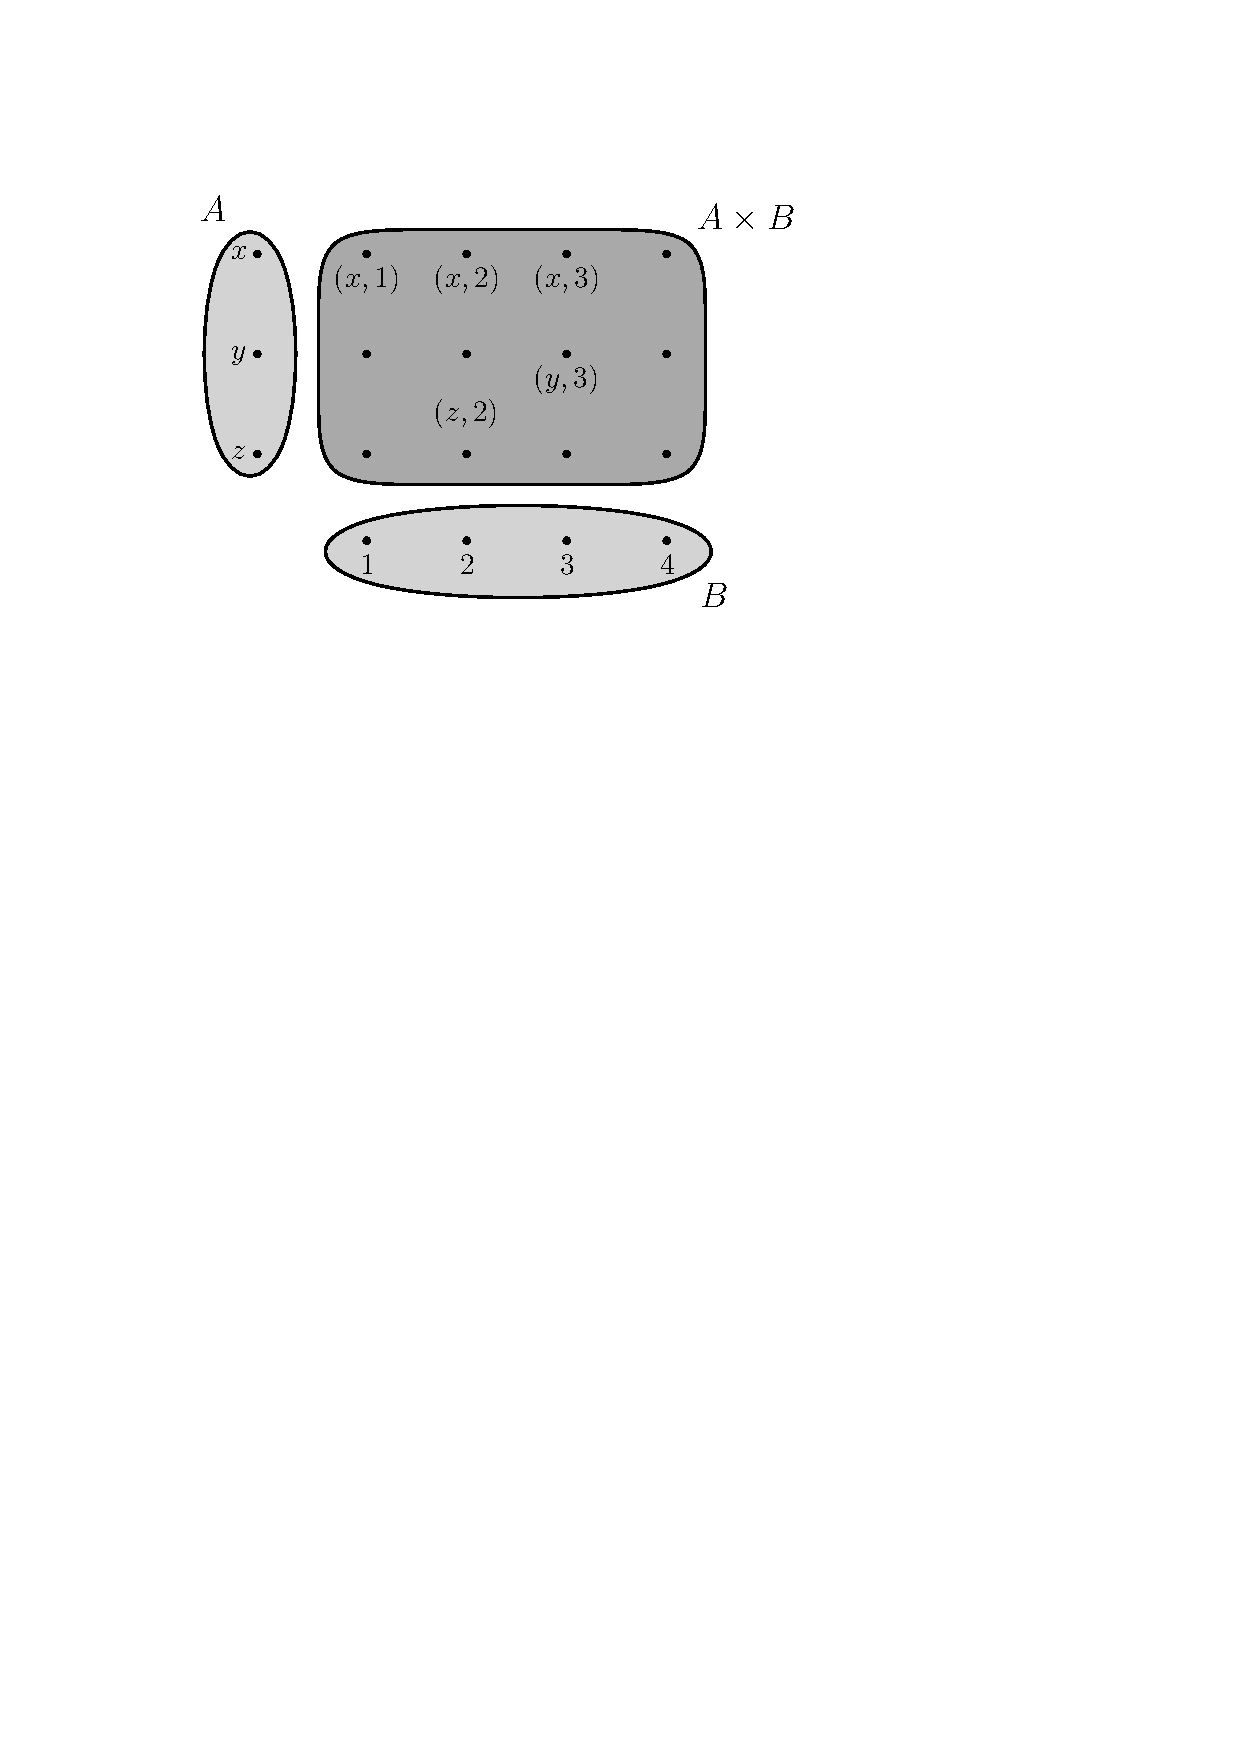
\includegraphics[scale=\normalipe]{ch02_kartezsky_soucin.pdf}
    \caption{Grafické znázornění kartézského součinu z příkladu \ref{ex:kartezsky_soucin}.}
    \label{fig:kartezsky_soucin}
\end{figure}
Pokud budeme však pracovat např. s intervaly reálných čísel, pak již nemůžeme takto kartézský součin znázornit, ale můžeme reprezentovat uspořádané dvojice jako body v~rovině. Např. pro $A=(2, 6\rangle$ a $B=\langle 1,3 \rangle$ je grafické znázornění na obrázku \ref{fig:kartezsky_soucin_intervaly}.
\begin{figure}[H]
    \centering
    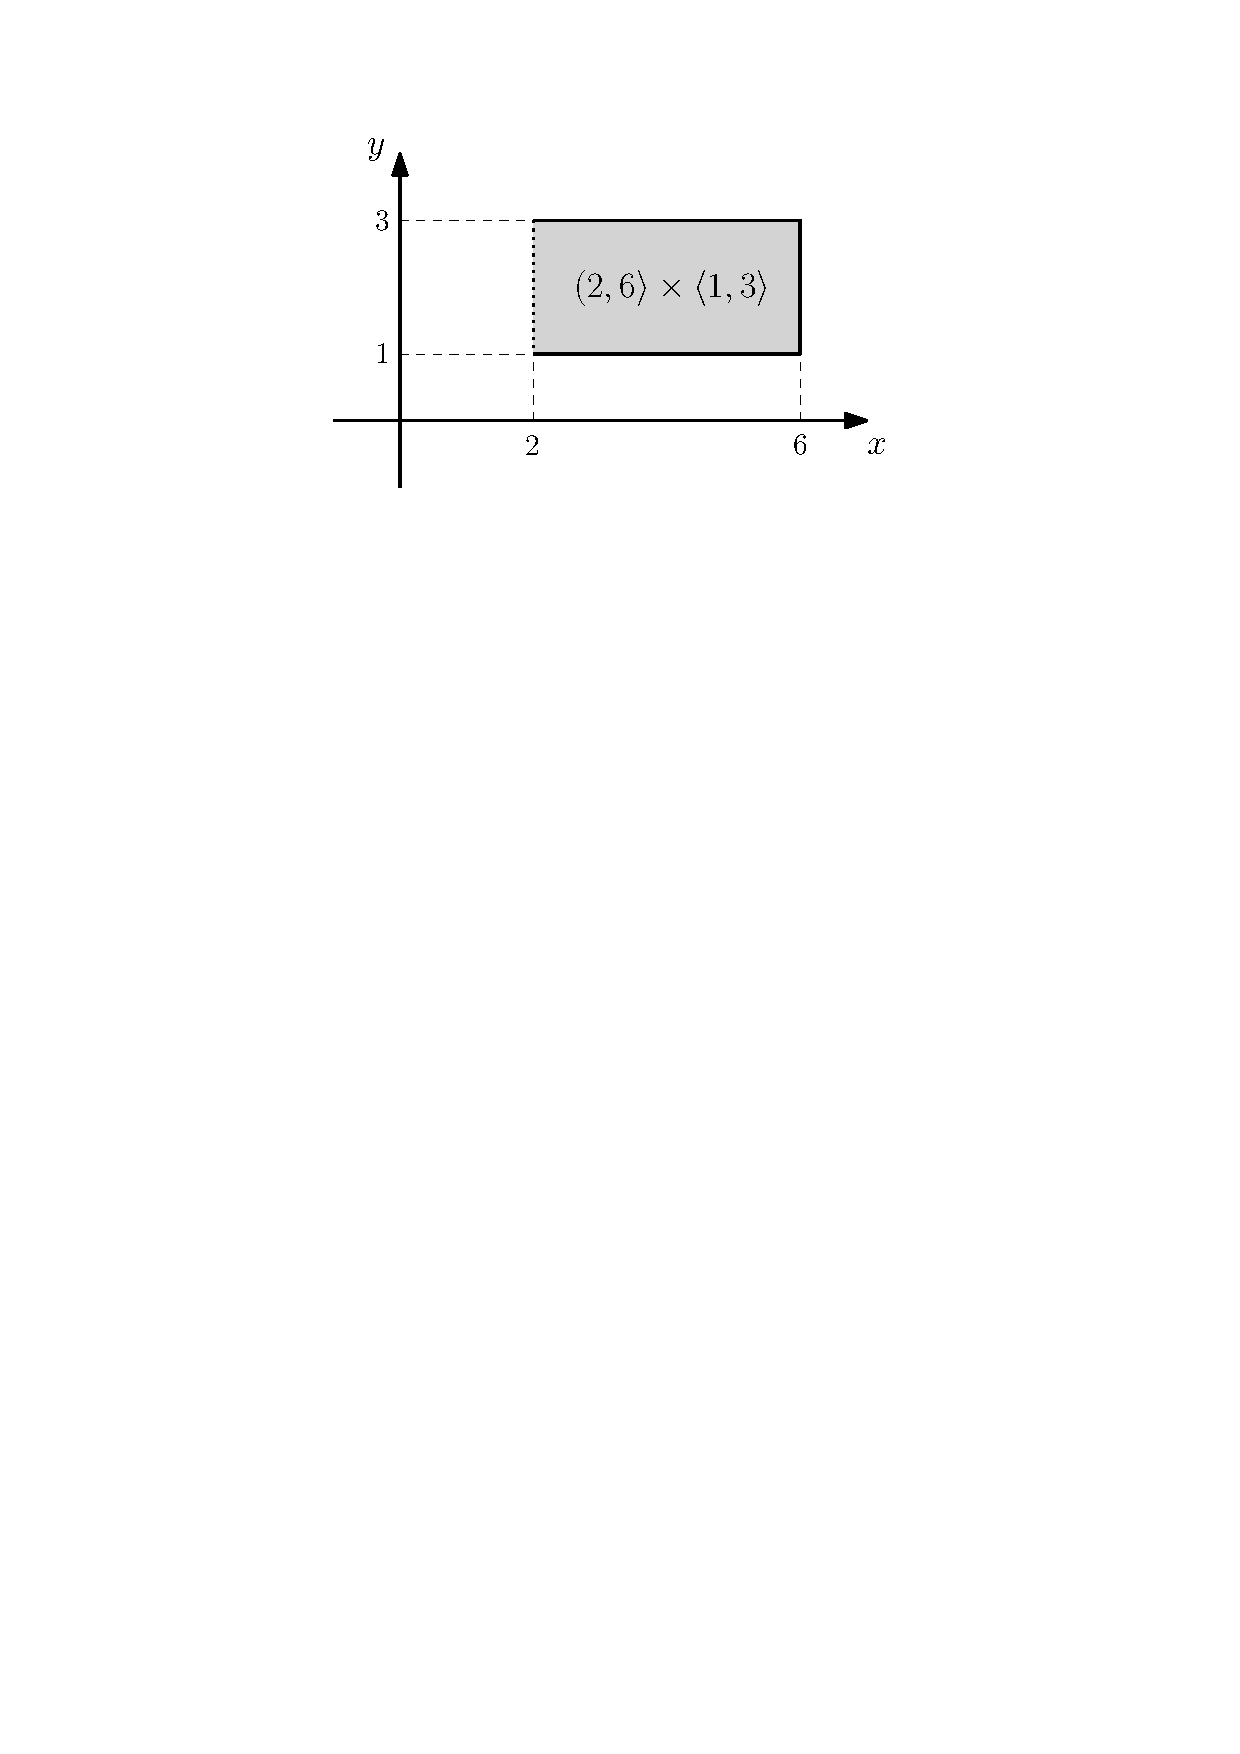
\includegraphics[scale=\normalipe]{ch02_relace_mezi_mnozinami_intervaly.pdf}
    \caption{Grafické znázornění kartézského součinu intervalů $(2, 6\rangle$ a $\langle 1,3 \rangle$.}
    \label{fig:kartezsky_soucin_intervaly}
\end{figure}
Podobně jako v~případě součinu čísel, i zde můžeme kartézské součiny stejných množin značit pomocí horního indexu (tzv. \emph{kartézské mocniny}), např. $A\times A=A^2$, $A\times A\times A=A^3$, atd. Obecně lze definovat
\begin{align*}
    A^1=A,\\
    A^n=A^{n-1}\times A.
\end{align*}
Neplatí zde však asociativní ani komutativní zákon:
\begin{align*}
    (A\times B)\times C&\neq A\times (B\times C),\\
    A\times B&\neq C\times A,
\end{align*}
protože jak jsme si již dříve uvedli, tak obecně $(x,y)\neq (y,x)$. (Zkuste si rozmyslet.)
\begin{example}
    Nechť je dána množina $X=\set{a,b}$. Vypočítejte $X^3$.
\end{example}
\begin{solution}
    Kartézský součin $X^3$ můžeme vypočítat jako $X^2\times X$.
    \begin{equation*}
        X^2=\set{(a,a),\,(a,b),\,(b,a),\,(b,b)}
    \end{equation*}
    Nyní stačí dopočítat $X^2\times X=X^3=\set{(a,a),\,(a,b),\,(b,a),\,(b,b)}\times\set{a,b}$, čímž obdržíme
    \begin{align*}
        X^3=&\{(a,(a,a)),\,(a,(a,b)),\,(a,(b,a)),\,(a,(b,b)),\,(b,(a,a)),\,(b,(a,b)),\,(b,(b,a)),\\
        &(b,(b,b))\}.
    \end{align*}
    Ovšem jak jsme již zmiňovali, tak $(x,(y,z))=(x,y,z)$, tedy množina $X^3$ jednoduše obsahuje všechny uspořádané trojice prvků z $x$.
    \begin{equation*}
        X^3=\set{(a,a,a),\,(a,a,b),\,(a,b,a),\,(a,b,b),\,(b,a,a),\,(b,a,b),\,(b,b,a),\,(b,b,b)}.
    \end{equation*}
\end{solution}